\section{Model}
The different tasks that have to be accomplished when playing a complete game of Starcraft could be grouped into an hierarchy as in Figure \ref{conceptualModel}. This somewhat captures the way human think about the entities of the game when playing.

\begin{figure}[h!t]
\centering
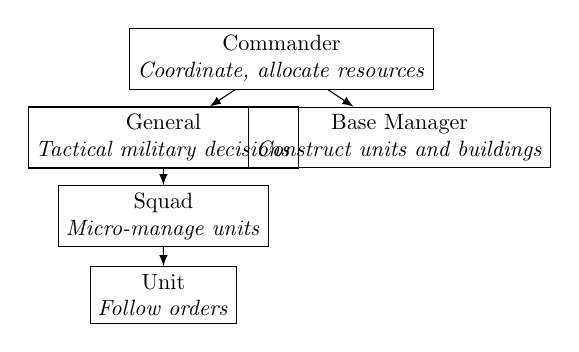
\begin{tikzpicture}[node distance = 1 cm]
    \tikzstyle{quadri}=[rectangle,draw, align=center, scale=0.8]
    \tikzstyle{link}=[->,thin,>=latex]
    \node[quadri] (commander) at (0,2) {Commander \\ \emph{Coordinate, allocate resources}};
    \node[quadri] (general) at (-1.5,1) {General \\ \emph{Tactical military decisions}};
    \node[quadri] (squad) at (-1.5,0) {Squad \\ \emph{Micro-manage units}};
    \node[quadri] (unit) at (-1.5,-1) {Unit \\ \emph{Follow orders}};
    \node[quadri] (basemanager) at (1.5,1) {Base Manager \\ \emph{Construct units and buildings}};
    \draw[link] (commander)--(general);
    \draw[link] (general)--(squad);
    \draw[link] (squad)--(unit);
    \draw[link] (commander)--(basemanager);

\end{tikzpicture}
\caption{
\emph{Conceptual model} of the high level task involved in playing a complete game of Starcraft. All actors in this hierarchy are virtual except for the units.
}
\label{conceptualModel}
\end{figure}

\begin{definition}[Commander]
One per game. Decides how the available resources should be allocated between expanding the base to enable harvesting new resources even faster, and towards producing military units to defend and attack.
\end{definition}
\begin{definition}[Base Manager]
One per game. Constructs what the Commander wants, possibly given priorities.
\end{definition}
\textbf{}\begin{definition}[General]
One per game. Splits the available military units up into squads and assigns them objectives such as \texttt{Attack}, \texttt{Defend} and \texttt{Flee}.
\end{definition}
\begin{definition}[Squad]
As many as the general wants. They have a military goal and micro-manage every move of each unit.
\end{definition}
\begin{definition}[Unit]
The actual units in the game, ordered according to the wishes of the squad manager.
\end{definition}
